\documentclass[10pt]{article}
\usepackage[utf8]{inputenc}
\usepackage{graphicx}
\usepackage{url}
\usepackage{color}
\usepackage{amsmath}
\usepackage{pgf}
\usepackage{hyperref}
\usepackage{float}
\usepackage{fancyhdr}

\newtheorem{question}{Question}

\setlength {\parskip}{2mm}
\setlength {\parindent}{0mm}
\addtolength{\topmargin}{-2.5cm}
\addtolength{\textheight}{4cm}
\addtolength{\evensidemargin}{-20mm}
\addtolength{\oddsidemargin}{-20mm}
\addtolength{\textwidth}{40mm}
\thispagestyle{empty}
\pagestyle{empty}
\usepackage{graphicx}


\begin{document}

{\flushright \small \tt Master Bioinformatique parcours MISO 2021-22}

\begin{center}
\textbf{M\'ethodes pour l'Analyse Bioinformatique des S\'equences}

\end{center}


\hrule

\bigskip

\begin{center}

\textbf{\Large Projet 1: prédiction de gènes dans un génome bactérien}    
\end{center}

\bigskip

L'objectif de ce projet est de développer un programme en Python qui permette d'identifier les gènes codant pour des protéines dans un génome bactérien nouvellement séquencé et assemblé. 


La première étape, présentée en section 1, repose sur la recherche des ORF ({\em open reading frames}), la deuxième étape, présentée en section 2, sur une approche statistique qui exploite le biais de composition en triplets. Enfin, en section 3, nous vous proposons d'affiner les prédictions en identifiant les motifs RBS souvent présents en amont des ORF ({\em Ribosome Binding Sites}).

Pour rappel, une ORF est une suite de codons commençant par un codon START, terminant par un codon STOP dans la même phase et ne comprenant pas de codon STOP intermédiaire. Notez bien, par contre, qu'une ORF peut contenir des codons START intermédiaires.

D'un point de vue informatique, dans tout le projet, une ORF est caractérisée par 

\begin{itemize}
\item une position de début sur le génome;
\item une position de fin sur le génome;
\item le brin, $+$ ou $-$.
\end{itemize}

Les positions de début et de fin sont relatives au brin $+$ du génome. Quand l'ORF est sur le brin $+$, la position de début est celle du codon START et la position de 
fin est celle du codon STOP. Inversement, quand l'ORF est sur le brin $-$, la position de début est celle du codon STOP et la position de fin est celle du codon START.


Le programme, nommé {\tt Simple\_ORF\_finder.py},  acceptera en arguments de la ligne de commande les paramètres obligatoires suivants: 
\begin{itemize}
\item {\tt -i (--infasta)} : fichier fasta du génome à analyser 
\item {\tt -c (--counttable)} : table de comptage des codons 
\item {\tt -t (--codonstable)} : code génétique utilisé pour la traduction
\item{\tt  -o (--outgff)} : nom d'un fichier de sortie au format GFF
\end{itemize}
En paramètre optionnel:
\begin{itemize}
\item {\tt -s (--minorfsize)} : taille minimum des ORFs. Par défaut, la valeur est 300.   
\end{itemize}

Les objets {\tt DnaSeq} et {\tt OrfSeq} (figure \ref{fig:class_diag}) seront implémentés dans un fichier à part {\tt Seq.py} puis importés dans le programme principal.

Pour faire des tests, nous vous fournissons deux fichiers:
\begin{itemize}
    \item Fichier fasta: {\tt GCF\_000009045.1\_ASM904v1\_partial\_genomic.fna}
    \item Table de comptage: {\tt E\_coli\_K12\_MG1655\_CDS\_table}, issue de régions codantes connues chez {\em E. Coli}
    \item Code génétique: {\tt code\_genetique\_bacteries}  % A quoi sert cette table ? Mathieu => c'est pour qu'il aient la correspondance entre les codon synonymes et les AA... ils pourront l'implémenter dans le programme...
\end{itemize}

Pour information, le code génétique utilisé est celui de la table 11 (\href{https://www.ncbi.nlm.nih.gov/Taxonomy/Utils/wprintgc.cgi}{disponible ici}) "Bacterial, Archaeal and Plant Plastid Code":

\begin{itemize}
    \item codons START : 'ATG','GTG','TTG','ATT','ATC','ATA','CTG'
    \item codons STOP : 'TGA','TAA','TAG'
\end{itemize}

Votre code devra être commenté, documenté (docstrings) et respecter les conventions de codage.

\section{Détermination et affichage des ORF}

\begin{question}
Écrire une fonction {\tt parseFasta(Fi)} qui prend en entrée un fichier {\tt Fi} contenant une séquence d’ADN au format Fasta et en extrait son identifiant et sa description (première ligne) ainsi que la séquence  (deuxième ligne jusqu'au prochain identifiant). Cette fonction devra gérer correctement les erreurs de syntaxe, c’est-à-dire le cas où le fichier ne contient pas les informations au format attendu.
Chaque séquences sera stockée dans un objet {\tt DnaSeq} (figure \ref{fig:class_diag}).
Cette fonction devra retourner une liste d'objets {\tt DnaSeq}.
\end{question} 


\begin{question}
Écrire une méthode {\tt computeORF(l)} qui détermine toutes les ORF de longueur supérieure ou égale à l'argument {\tt l}. Chaque ORF sera stockée dans un objet {\tt OrfSeq} (figure \ref{fig:class_diag}), classe fille de {\tt DnaSeq}.
Les ORF devront être triées par ordre croissant de leur position de début.

Utilisez le code génétique fournis {\tt code\_genetique\_bacteries} pour en extraire les codons Start et Stop.
\end{question}

\begin{question} 
Écrire une fonction {\tt displayORF(debutIntervalle,finIntervalle)}  qui prend en entrée un couple de positions {\tt debutIntervalle} et {\tt finIntervalle}, et affiche toutes les ORF dont la position de début est comprise dans l'intervalle de positions {\tt [debutIntervalle..finIntervalle]}. Pour être efficace, cette fonction exploitera le fait que les ORF sont triées. La
détermination de la première ORF de l'intervalle se fera ainsi avec une recherche dichotomique dans le tableau des ORF.
Chaque ligne correspondra à une ORF dont les informations seront affichées au format \href{https://fr.wikipedia.org/wiki/General_feature_format}{GFF}. Le format à respecter pour les lignes est le suivant:

{\tt chromosome\_ID<tab>Nom\_du\_programme<tab>gene<tab>start<tab>end<tab>score<tab>brin<tab>phase}

avec:
\begin{itemize}
    \item {\tt <tab>} = tabulation
    \item {\tt chromosome\_ID} = l'identifiant du chromosome/scaffold où se trouve l'ORF
    \item {\tt Nom\_du\_programme}= {Simple\_ORF\_finder}
\end{itemize}

\end{question} 

\begin{figure}[H]
    \centering
    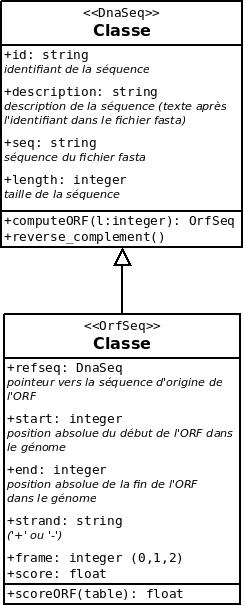
\includegraphics[scale=0.6]{Diagramme_UML_v1.jpeg}
    \caption{Diagramme de classe du projet pour la bibliothèque Seq.py}
    \label{fig:class_diag}
\end{figure}

\section{Utilisation du biais de composition en codons}

La redondance du code génétique implique que la plupart des acides aminés sont codés par plusieurs codons synonymes (64 codons possibles pour 20 acides aminés). L’usage des codons synonymes n’est pas aléatoire, la fréquence est différente que l’on se trouve au niveau du génome, dans les gènes fonctionnellement liés et au sein de gènes uniques. On parle alors de {\em biais dans l'usage des codons}. Généralement les gènes les plus exprimés sont les plus biaisés, les codons les plus utilisés étant ceux pour lesquels les ARN de transfert sont les plus nombreux (codons sélectionnés pour une plus grande vitesse de traduction).
Il est ainsi possible d’utiliser cette propriété pour rechercher parmi un ensemble d’ORF potentielles, celles dont les biais d’usage se rapprochent des valeurs calculées à partir d’un ensemble de gènes connus.

Cette observation permet d'aider à la prédiction de gènes en discriminant les séquences codantes des séquences non codantes sur la base de leur composition en codons.
Nous vous fournissons une table d'usage du code dans le fichier {\tt E\_coli\_K12\_MG1655\_CDS\_table}. Cette table, composée de 2 colonnes (codon, comptage) a été générée à partir de séquences codantes du génome d'{\em E. coli}.

A partir de cette table et du code génétique fournis {\tt code\_genetique\_bacteries}, on peut générer la matrice d'{\em utilisation relative des codons synonymes} (RSCU) qui servira de référence pour calculer le score des ORF. Le RSCU, noté $r$, calcule l’usage relatif des codons par rapport à un usage uniforme. Pour tout acide aminé $A$ et pour tout codon $i$ qui code pour A, $ri$  est défini par l'équation (\ref{eq:eq_rscu}).

\begin{equation} \label{eq:eq_rscu}
    %r_{i}=\frac{C_{i}}{(\frac{1}{d_{A}} \sum_{k \in cod(A)} C_{k}) }
    r_{i}=d_{A}\frac{C_{i}}{\sum_{k \in cod(A)} C_{k}}
\end{equation}

avec:
\begin{itemize}
\item $d_{A}$: le nombre de codons synonymes pour l’acide aminé $A$
\item $C_{i}$: le comptage pour le codon $i$
\item $cod(A)$: l’ensemble des codons synonymes pour l’acide aminé $A$
\end{itemize}

Si $r = 1$ le codon est utilisé comme attendu. Si $r < 1$ il est moins utilisé, et inversement si $r > 1$. 
Par exemple, la cystéine est codée par 2 codons {\tt TGT} et {\tt TGC}. 
S'il n’y avait pas de biais d’usage, on s’attendrait à avoir une fréquence de $0.5$ pour chacun des deux codons. 
Si on observe un comptage de $25$ pour {\tt TGT} et $75$ pour {\tt TGC}, on calcule $r_{TGT}= 0,5$ et  $r_{TGC}= 1,5$
On a donc  $r_{TGT}<1$ qui est le codon le moins utilisé, et  $r_{TGC}>1$ qui est le codon le plus utilisé.


Pour calculer le score $S_{orf}$ d'une séquence $S$, il suffit de calculer la somme (\ref{eq:eq_score}) des $(r_{i} - 1)$ de tous les codons  composant la séquence 

\begin{equation} \label{eq:eq_score}
    % S_{orf}(S)=log_{2}(\prod_{i\in S} r_{i}^\frac{1}{L}) 
    % => Hélène S_{orf}(S) = \sum_{i\in S} r_i % à vérifier
    S_{orf}(S) = \sum_{i\in S} (r_i-1)
    % Mathieu => j'ai testé, en effet la somme des ri fonctionne mieux pour la prédiction...
\end{equation}
Ainsi, si le score $r_{i} < 1$ on ajoute une pénalité négative au score et inversement, si $r_{i} > 1$.
\begin{question}
Écrire une méthode {\tt scoreORF(table)} dans la classe {\tt OrfSeq} (figure \ref{fig:class_diag}), qui prend en argument une {\tt table} d'usage du code et calcule le score sur la séquence de l'objet {\tt OrfSeq}.
Écrire ensuite une fonction {\tt computeORFscore()} qui calcule le score de chaque ORF et retourne, une liste d'objets {\tt OrfSeq} .
\end{question}

Pour continuer à affiner la prédiction de gènes, on cherche à éliminer les ORF {\em chevauchantes}, c'est-à-dire les ORF qui partagent des positions en commun (qu'elles soient ou pas sur le même brin). L'idée est de calculer le sous-ensemble, ou la combinaison, d'ORF non-chevauchantes qui soit maximal vis-à-vis du score défini juste au-dessus.

\begin{question}
Écrire une fonction {\tt maximiseORFscore()} qui étant donné un tableau d'ORF triées munies de leur score $S_{ORF}$ calcule le sous-ensemble des ORF non-chevauchantes de score total maximum. Pour cela, on pourra utiliser la programmation dynamique, en définissant $SORF(i)$ comme le score total maximum des ORF. Pour répondre à la question, il faut donc commencer par écrire une formule de récurrence pour $SORF(i)$, puis l'implémenter avec une table et enfin reconstruire la combinaison optimale à partir de la table.

Enfin, en vous aidant de la fonction écrite à la question 3, écrire dans un fichier de sortie GFF (argument --outgff) l'ensemble des ORF retenues triées par position de départ.
\end{question}

\section{Question Bonus - recherche du motif RBS}
La grande difficulté dans la recherche des ORF demeure la localisation des codons initiateurs des régions codantes.
Chez les procaryotes, l'initiation de la traduction se fait après association du ribosome avec une région contenant un site de fixation pour la petite sous unité du ribosome. Cette région (Ribosome Binding Site ou RBS) renferme une séquence complémentaire de l'extrémité 5' de l'ARN 16S. Cette séquence contient généralement le motif GGAGA situé à 6 ou 11 bases du codon initiateur (des distances plus grandes ou plus petites ont été observées).

Pour affiner la prédiction des gènes, on pourra rechercher en amont de chaque ORF la présence de cette région. Cette étape devra être effectuée avant le calcul des scores.

\begin{question}
Écrire une méthode {\tt rechercheRBS()} dans la classe {\tt OrfSeq} qui permet de rechercher la présence du site de fixation (RBS) à une distance située entre 5 et 15 bases en amont du codon initiateur ainsi qu'un seuil de 4.5 pour le score du motif. Cette méthode retournera un booléen True/False en fonction de la présence/absence de cette séquence.

\begin{figure}[ht]
\centering
{\tt [MOTIF\ RBS]<--\ 5\ à\ 15\ bases\ -->[CODON\ START]}
\end{figure}

Afin de tenir compte des variation que l'on peut avoir à chaque position du motif, vous réaliserez la recherche à l'aide de la matrice de poids donnée en figure \ref{fig:matr_ggagg} et dans le fichier {\tt $matrice\_GGAGA\_RBS\_E\_coli$}, établie sur un ensemble de séquences connues et représentant mieux cette variation.
\begin{figure}[ht]
\centering
$
\begin{matrix}
A & C & G & T\\
-3.88 & -13.30 & 2.00 & -13.30\\
-13.30 & -0.31 & 1.76 & -13.30\\
1.14 & 0.18 & -13.30 & -1.09\\
0.51 & -13.30 & 1.25 & -13.30\\
0.79 & 0.12 & -13.30 & 0.08
\end{matrix}
$
\caption{matrice de poids {\tt GGAGA} pour E. coli - score seuil = 4.5}
\label{fig:matr_ggagg}
\end{figure}

Écrire une fonction {\tt computeRBS()} qui détermine la présence/absence du site de fixation pour chaque ORF et retourne, dans une liste d'objets {\tt OrfSeq}, les ORF pour lesquels le motif est détecté en amont. 

\end{question}

\end{document}
